\section{Actividad 4}

\subsection*{Graficar las señales senoidales correspondientes que cumplan las siguientes condiciones:}

\subsubsection*{a) Señal de amplitud \(A\) aleatoria uniforme, distribuida entre \([8, 40]\).}

\[
x(t) = A \cos(2 \pi 10 t)
\]

La gráfica muestra una señal con amplitud modulada aleatoriamente en cada $t$, oscilando entre aproximadamente $-40$ y $40$, con una frecuencia base de 10 Hz. La variabilidad de $A$ crea una envolvente irregular alrededor de la senoidal. La autocorrelación presenta un pico máximo cercano a 125000 en $\tau=0$, con oscilaciones a 10 Hz que decaen gradualmente, reflejando la modulación aleatoria. En una senoidal pura con $A \approx 19.99$ fijo, la señal oscilaría entre $\pm 19.99$, y la autocorrelación sería más regular.

\begin{figure}[H]
\centering
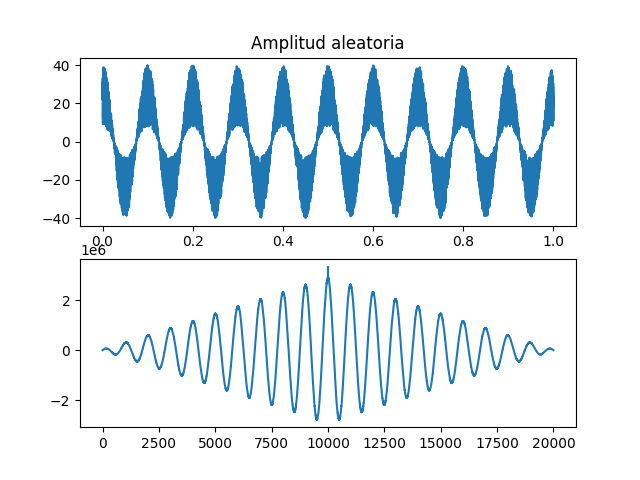
\includegraphics[width=0.8\textwidth]{imagenes/Actividad_4/senal_a.png}
\caption{Señal con amplitud aleatoria y su autocorrelación.}
\label{fig:a}
\end{figure}

\subsubsection*{b) Señal de fase \(\Theta\) aleatoria uniforme, distribuida entre \([-\pi, \pi]\).}

\[
x(t) = 5 \cos(2 \pi 10 t + \theta)
\]

La gráfica muestra una señal con amplitud constante de 5, modulada por una fase variable en cada $t$ dentro de $[-0.25\pi, 0.25\pi]$, resultando en una senoidal de 10 Hz con distorsiones. La autocorrelación tiene un pico máximo cercano a 12500 en $\tau=0$, con oscilaciones a 10 Hz que decaen, afectadas por la variabilidad de $\theta$. En una senoidal pura con $\theta \approx 2.83$ rad fijo, la señal sería una senoidal desplazada, y la autocorrelación sería más uniforme.

\begin{figure}[H]
\centering
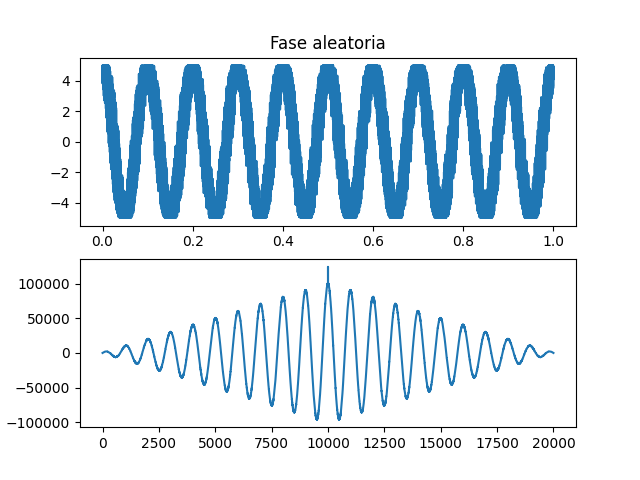
\includegraphics[width=0.8\textwidth]{imagenes/Actividad_4/senal_b.png}
\caption{Señal con fase aleatoria y su autocorrelación.}
\label{fig:b}
\end{figure}

\subsubsection*{c) Señal de frecuencia \(f\) aleatoria uniforme, distribuida entre \([0, 20]\).}

\[
x(t) = 5 \cos(2 \pi f t)
\]

La gráfica muestra una señal con amplitud constante de 5, pero con frecuencia variable en cada $t$ dentro de $[3, 20]$ Hz, resultando en una forma de onda no periódica que parece ruido, oscilando entre aproximadamente $-4$ y $4$. La autocorrelación presenta un pico máximo cercano a 125000 en $\tau=0$, con una estructura difusa debido a la variabilidad de $f$. En una senoidal pura con $f \approx 14.64$ Hz fijo, la señal tendría $\approx 14.64$ ciclos en 1 s, y la autocorrelación mostraría oscilaciones claras a esa frecuencia.

\begin{figure}[H]
\centering
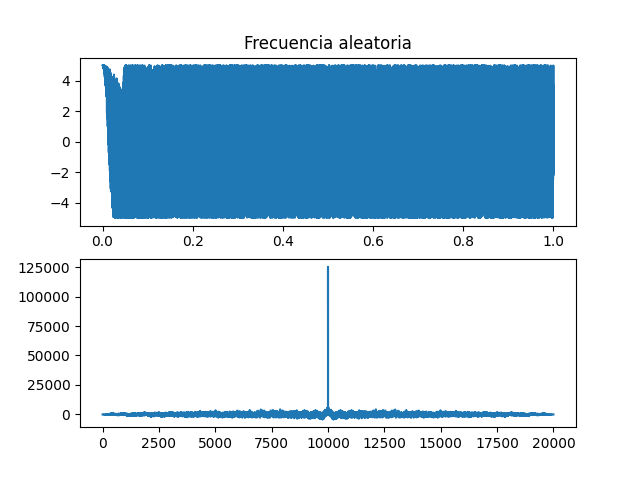
\includegraphics[width=0.8\textwidth]{imagenes/Actividad_4/senal_c.png}
\caption{Señal con frecuencia aleatoria y su autocorrelación.}
\label{fig:c}
\end{figure}

\subsubsection*{d) Señal de amplitud, fase y frecuencia aleatoria, distribuidas de igual forma que los puntos anteriores.}

\[
x(t) = A \cos(2 \pi f t + \theta)
\]

La gráfica combina las modulaciones aleatorias de $A$ (en $[8, 40]$), $\theta$ (en $[-0.25\pi, 0.25\pi]$) y $f$ (en $[3, 20]$), resultando en una señal altamente distorsionada que oscila entre aproximadamente $-40$ y $40$. La autocorrelación tiene un pico máximo cercano a 3 en $\tau=0$, con una estructura ruidosa y sin periodicidad clara debido a la combinación de variabilidades. En una senoidal pura con $A \approx 19.99$, $\theta \approx 2.83$ rad y $f \approx 14.64$ Hz, la señal sería una senoidal clara, y la autocorrelación reflejaría la frecuencia de 14.64 Hz.

\begin{figure}[H]
\centering
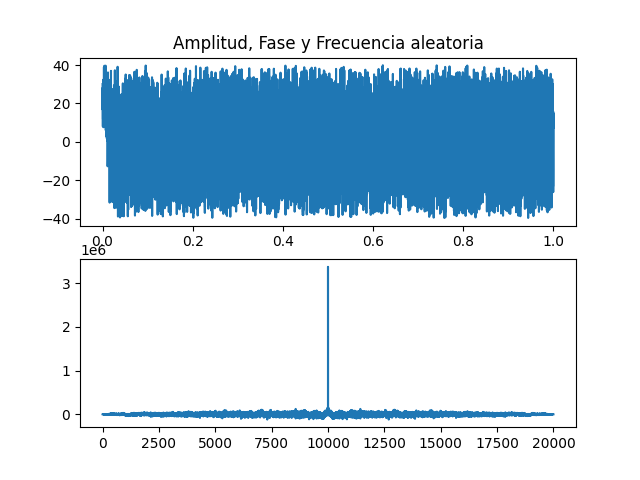
\includegraphics[width=0.8\textwidth]{imagenes/Actividad_4/senal_d.png}
\caption{Señal con amplitud, fase y frecuencia aleatorias y su autocorrelación.}
\label{fig:d}
\end{figure}

\subsection*{Además, graficar la auto-correlación para todos los puntos anteriores. ¿Qué información se obtienen al observar la gráfica de auto-correlación?.}

La autocorrelación $R_{xx}(\tau)$ mide la similitud de $x(t)$ consigo misma en diferentes retardos $\tau$:

\[
R_{xx}(\tau) = \int_{-\infty}^{\infty} x(t) x(t + \tau) \, dt
\]

Para señales de duración finita (1 s), la autocorrelación tiene una envoltura triangular. Basado en las gráficas generadas:

\begin{itemize}
    \item \textbf{Frecuencia}: En (a) y (b), las autocorrelaciones muestran oscilaciones a 10 Hz, pero con ruido debido a la modulación aleatoria de $A$ y $\theta$. En (c) y (d), la variabilidad de $f$ elimina la periodicidad clara, resultando en autocorrelaciones difusas.
    \item \textbf{Energía}: El valor en $\tau=0$ es proporcional a la energía ($R_{xx}(0) = \int x^2(t) \, dt$). En (a) y (d), los picos (125000 y 3, respectivamente) reflejan la mayor amplitud variable, mientras que en (b) y (c) (12500 y 125000) corresponden a $A=5$ con modulación.
    \item \textbf{Fase}: La autocorrelación es invariante a $\theta$, pero la variabilidad en (b) y (d) introduce ruido que distorsiona esta propiedad.
    \item \textbf{Estructura}: Para senoidales puras, $R_{xx}(\tau)$ tendría oscilaciones cosenoidales claras dentro de una envoltura triangular. Las gráficas actuales muestran distorsiones debido al ruido introducido por parámetros variables.
\end{itemize}

En conclusión, las autocorrelaciones reflejan las propiedades energéticas de las señales, pero la modulación aleatoria en las gráficas generadas introduce ruido que oculta la periodicidad esperada en señales senoidales puras.